\chapter{Link-Cut Trees}
\newcommand{\key}{\operatorname{key}}
\newcommand{\prio}{\operatorname{prio}}

In this chapter, we will learn about a dynamic data structure that allows us to speed-up Dinic's algorithm even more: \emph{Link-Cut Trees}. This chapter is inspired by lecture notes of Richard Peng\footnote{CS7510 Graph Algorithms Fall 2019, Lecture 17 at \url{https://faculty.cc.gatech.edu/~rpeng/CS7510\_F19/}} and the presentation in a very nice book on data structures and network flows by Robert Tarjan \cite{tarjan1983data}.

\section{Overview}

\paragraph{Model.} We consider a directed graph $G=(V,E)$ that is undergoing \emph{updates} in the form of edge insertions and/or deletions. We number the graph in its different \emph{versions} $G^0, G^1, G^2, \dots$ such that $G^0$ is the initial input graph, and $G^i$ is the initial graph after the first $i$ updates were applied. Such a graph is called a \emph{dynamic} graph.

In this lecture, we restrict ourselves to \emph{dynamic rooted forests} that is we assume that every $G^i$ forms a directed forest where in each forest a single root vertex is reached by every other vertex in the tree. For simplicity, we assume that $G^0 = (V, \emptyset)$ is an empty graph.

\begin{figure}[!ht]
    \centering
    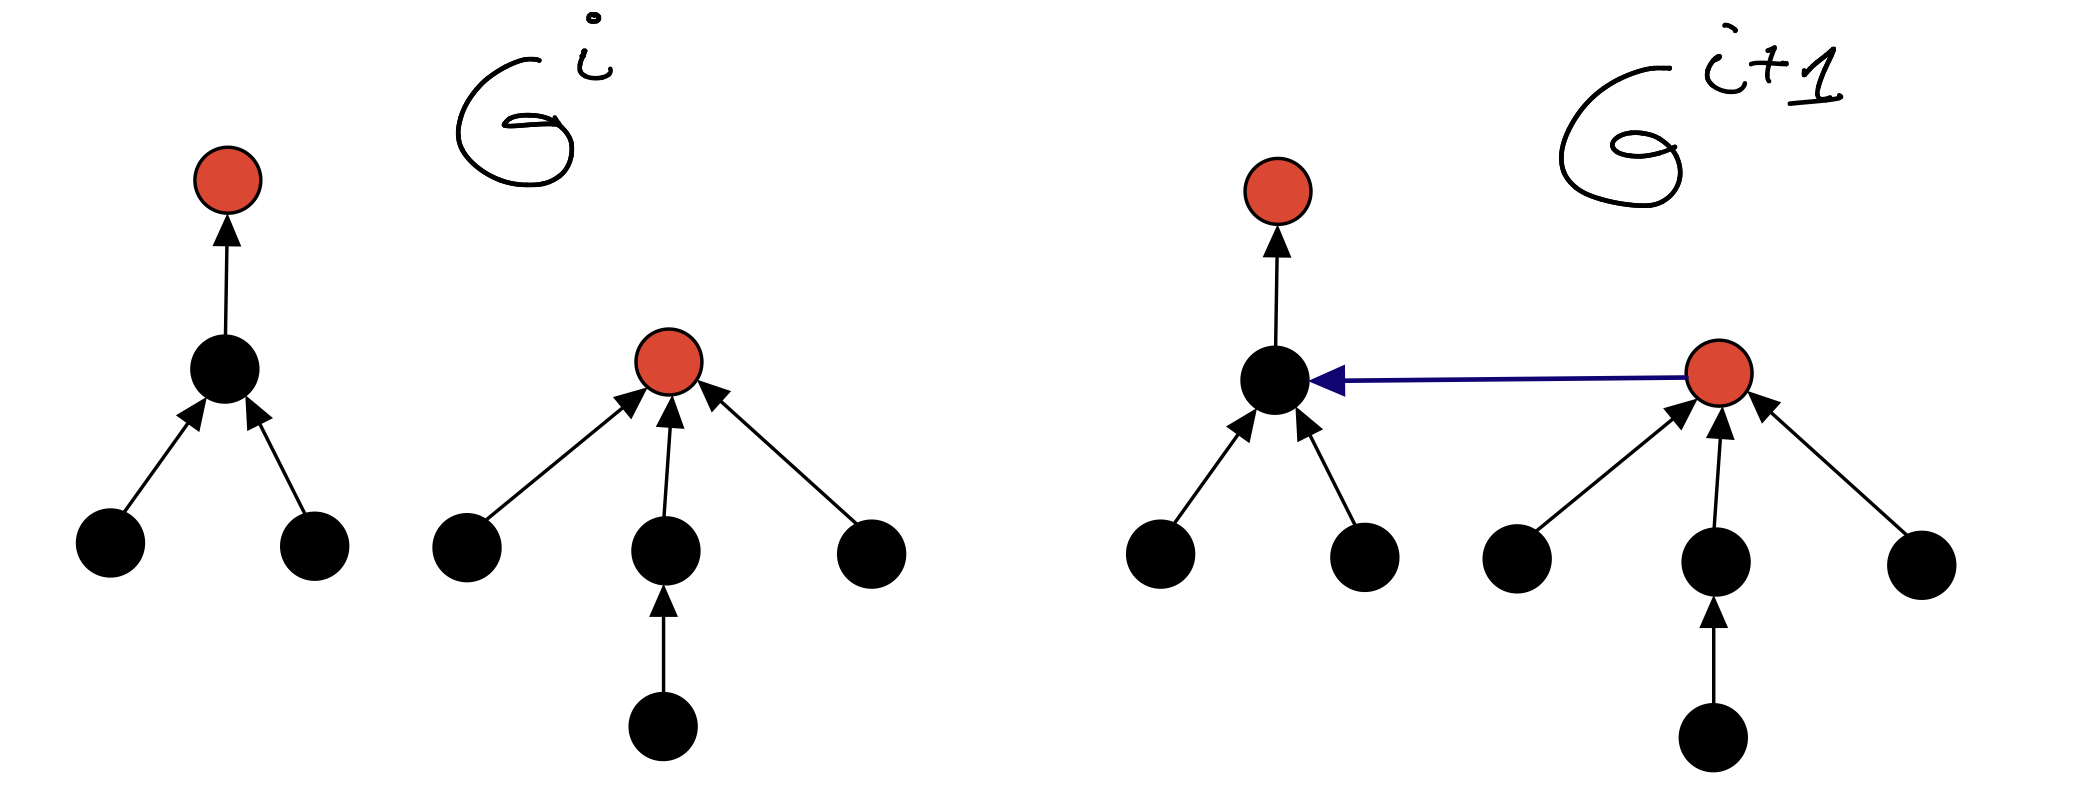
\includegraphics[scale=0.2]{./fig/InsertionDynamicTree_lectureDynamicTree.jpeg}
    \caption{The $i^{th}$ version of $G$ is a rooted forest. Here, red vertices are roots and there are two trees. The $(i+1)^{th}$ version of $G$ differs from $G^i$ by a single edge that was inserted (the blue edge). Note that edge insertions are only valid if the tail of the edge was a root. In the right picture, the former root on the right side is turned into a normal node in the tree by the update.}
    \label{fig:my_label}
\end{figure}

\paragraph{The Interface.} Let us now describe the interface of our data structure that we call a link-cut tree. We want to support the following operations:
\begin{itemize}
    \item $\textsc{Initialize}(G)$: Creates the data structure initially and returns a pointer to it. Each vertex is initialized to have an associated cost $cost(v)$ equal to $0$.
    \item $\textsc{FindRoot}(v)$: Returns the root of vertex $v$. 
    \item $\textsc{AddCost}(v, \Delta)$: Add $\Delta$ to the cost of every vertex on the path from $v$ to the root vertex $\textsc{FindRoot}(v)$.
    \item $\textsc{FindMin}(v)$: Returns tuple $(w, cost(w))$ where $w$ is the (first) vertex on the path from $v$ to $\textsc{FindRoot}(v)$ of lowest cost. 
    \item $\textsc{Link}(u,v)$: Links two trees that contain $u$ and $v$ into a single tree by inserting the edge $(u,v)$. This assumes that $u, v$ are initially in different trees and $u$ was a root vertex.
    \item $\textsc{Cut}(u,v)$: Cuts the edge $(u,v)$ from the graph which causes the subtree rooted at $u$ to become a tree and $u$ to become a root vertex. Assumes $(u,v)$ is in the current graph.
\end{itemize}

\paragraph{Main Result.} The following theorem is the main result of today's lecture.

\begin{theorem}\label{thm:mainTheoremLinkCutTree}
We can implement a link-cut tree such that any sequence of $m$ operations takes total expected time $O(m \log^2 n + |V|)$.
\end{theorem}


\section{Balanced Binary Search Trees: A Recap}
In \href{https://ti.inf.ethz.ch/ew/courses/APC21/Chapter_2.pdf}{Chapter 2 of the course Algorithms, Probability and Computing}, we introduced (balanced) binary search trees, and studied \emph{treaps}, which are a simple randomized approach to building a binary search tree with good performance, at least in expectation.
If you are not familiar with balanced binary search trees, we encourage you to read this chapter from the APC script. 
That said, we will quickly recap the important properties of binary search trees and treaps.
If you're already familiar with treaps, you can skip ahead to the next section to see how we use them for building Link-Cut trees.

A binary search tree $\mathcal{T}$ is a data structure for keeping track of a set of \emph{items} where each item has a \emph{key} associated with it.
The data structure stores the items in a rooted binary tree with a node for each item, and maintains the property for each node $v$, all items in the \emph{left} subtree of $v$ have keys less than $v$, and all items in the \emph{right} subtree of $v$ have keys greater than $v$.
This is called the \emph{search property} of the tree, because it makes it simple to search through the tree to determine if it contains an item with a given key.

The binary trees we studied in APC supported the following operations, while maintaining the search property:
\begin{description}
\item[insert:] We can add an item to the tree with a specified key.
\item[delete:] We can remove an item from the tree with a specified key.
\item[find:] Determine if the tree contains an item with a specified key.
\item[split:] Suppose the tree contains two items $v_1$ and $v_2$ with keys $k_1$ and $k_2$ where $k_1 < k_2$, and suppose no item in tree has a key $k$ in the interval $(k_1,k_2)$. Then the split operation applied to these two items should split the current tree into two: One tree containing all items with keys in $(-\infty,k_1]$ and the other with all items in $[k_2,\infty)$.
\item[join:] Given two binary search trees, one with keys in the interval $(-\infty,k]$, the other with keys in the interval $(k,\infty)$, form a single binary search tree containing the items of both.
\end{description}

\emph{Treaps} allow us to implement all of these operations, each with expected time $O(\log n)$ for each operation when working over $n$ items.

\paragraph{Tree rotations.} A crucial operation when implementing binary search trees in general and treaps in particular is \emph{tree rotation}. A tree rotation makes a local change to the tree by changing only a constant number of pointers around, while preserving the search property.
Given two items $v_1$ and $v_2$ such that $v_1$ is a child of $v_2$, a tree rotation applied to these two nodes will make $v_2$ the child of $v_1$, while moving their subtrees around to preserve the search property. This is shown in Figure~\ref{fig:binaryTreeRotation}.
When the rotation makes $v_2$ the right child of $v_1$ (because $v_2$ has the larger key), this is called a \emph{right rotation}, and when it makes $v_2$ the left child of $v_1$ (because $v_2$ has a smaller key), it is called a \emph{left rotation}.

\begin{figure}[H]
    \centering
    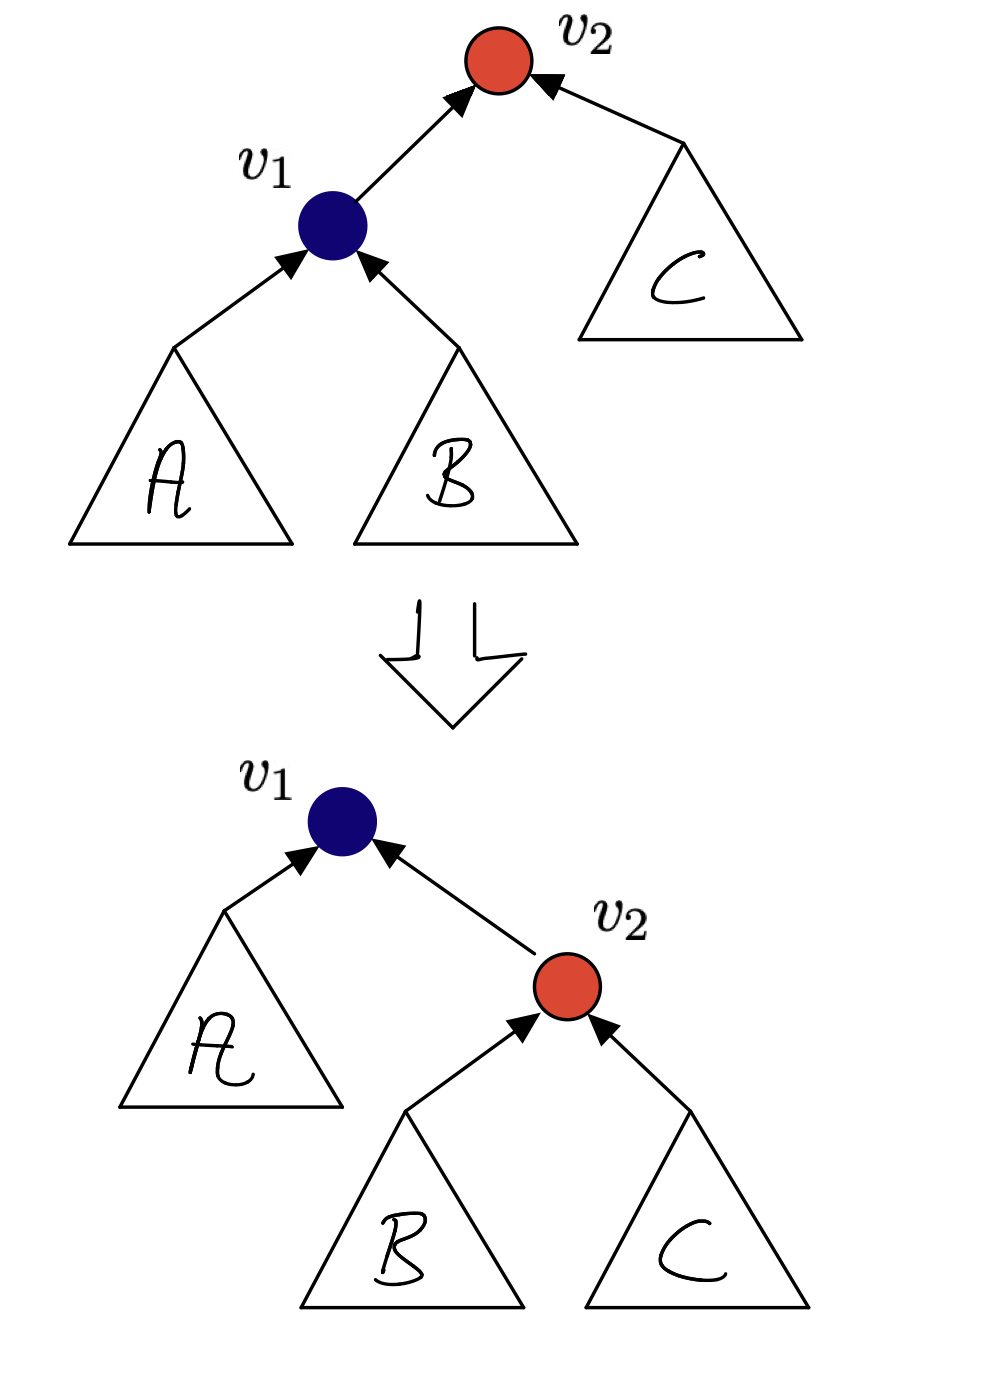
\includegraphics[scale=0.2]{./fig/TreeRotation_lectureDynamicTree.jpeg}
    \caption{Given two items $v_1$ and $v_2$ such that $v_1$ is a child of $v_2$, a tree rotation applied to these two nodes will make $v_2$ the child of $v_1$, while moving their subtrees around to preserve the search property. This figure shows a \emph{right rotation}.}
    \label{fig:binaryTreeRotation}
\end{figure}

\section{A Data Structure for Path Graphs}

Before we prove \Cref{thm:mainTheoremLinkCutTree} in its full generality, let us reason about implementing a link-cut tree data structure in a weaker setting: we assume that every version $G^i$ of $G$ is just a collection of rooted vertex-disjoint paths.

The treap now assigns a random \emph{priority} to each item, denoted $\prio(x)$.

\paragraph{Representing Paths via Balanced Binary Search Trees.} It turns out that paths can be represented rather straight-forwardly via Balanced Binary Search Trees. For the sake of concreteness, we here use \emph{treaps} to represent paths\footnote{If you have not seen treaps before, don't worry, they are simple enough to understand them from our application here. }. 

Let us describe how to represent a path $P$ in $G$. First, we pick for each vertex $v$, a random natural number $ranNum(v)$ uniformly at random from a large universe, say $[1, n^{100})$. We assume henceforth that $ranNum(v) \neq ranNum(w)$ for all $v,w\in V$.

Then, for each path $P$ in $G$, we store the vertices in $P$ in a binary tree $\mathcal{P}$ and enforce the invariants:
\begin{itemize}
    \item \textbf{Heap-Order}: for each vertex $v \in P$, its parent $w = parent_{\mathcal{P}}(v)$ in $\mathcal{P}$ is either $NULL$ (if $v$ is the root) or has $ranNum(v) > ranNum(w)$.
    \item \textbf{Search-Property}: for all $v$, $left_{\mathcal{P}}(v)$ precedes $v$ on $P$ and $right_{\mathcal{P}}(v)$ appears later on $P$ than $v$. See the picture below for an illustration.
\end{itemize}

\begin{figure}[!ht]
    \centering
    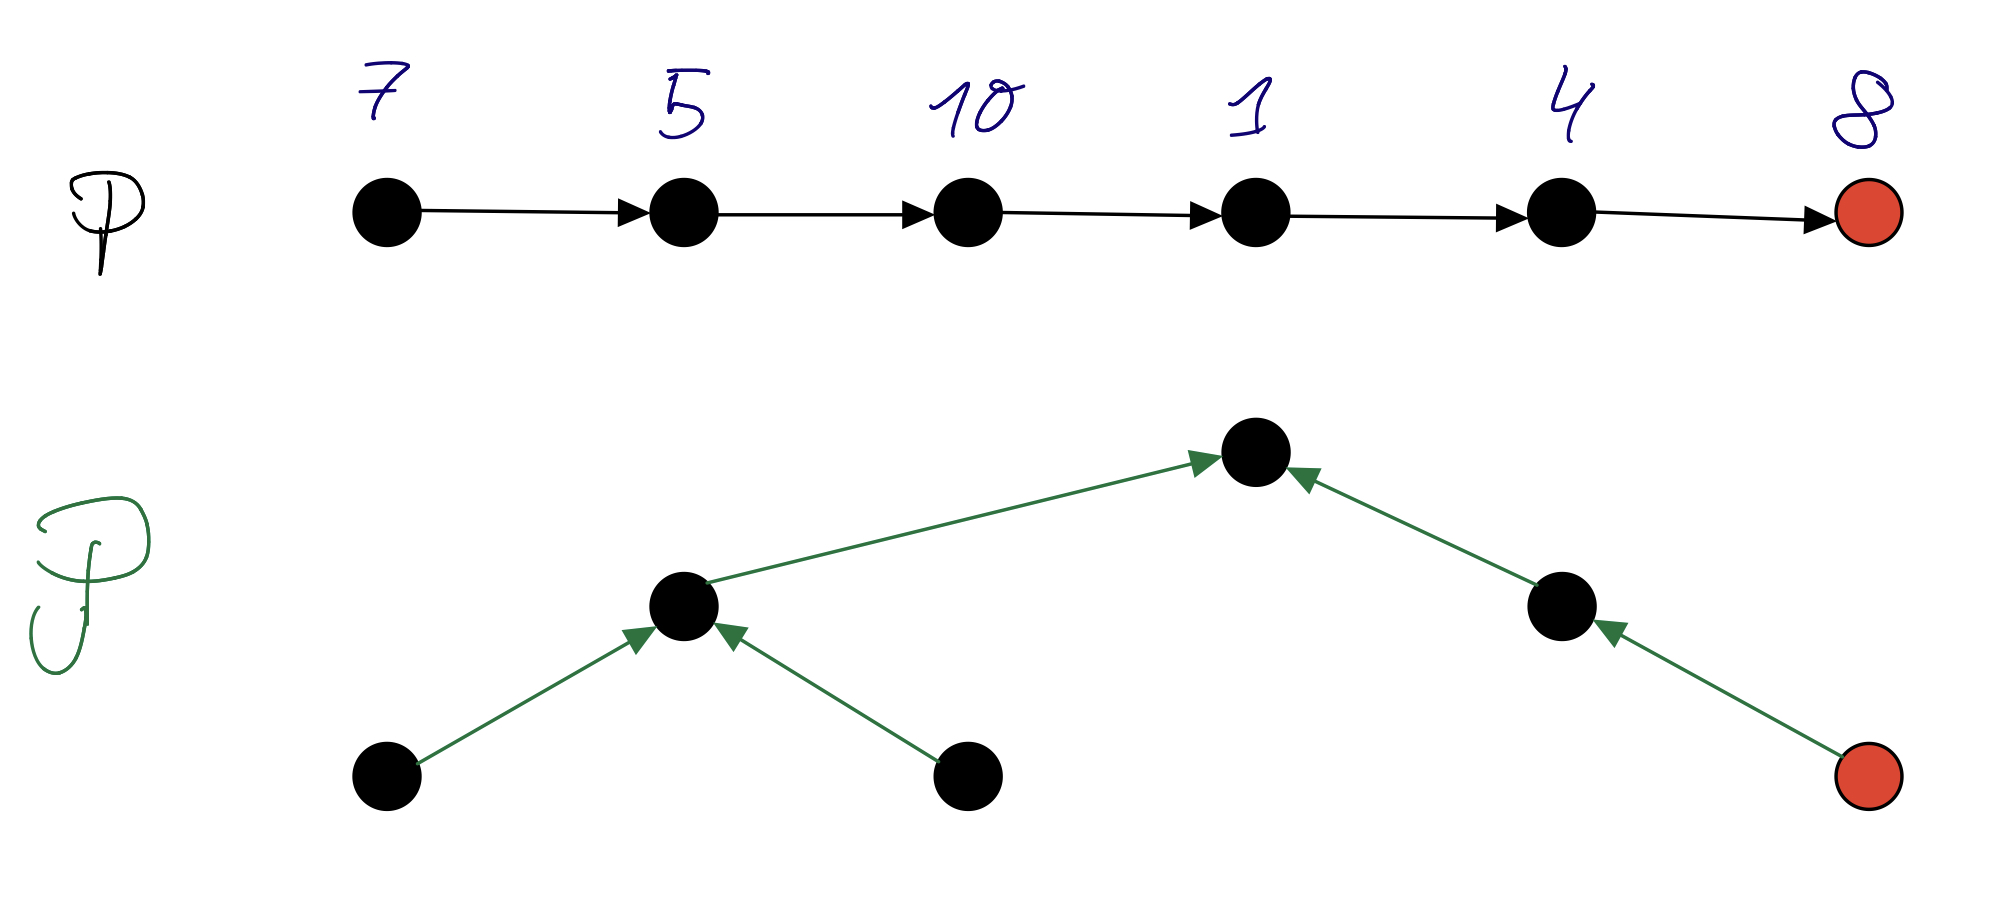
\includegraphics[scale=0.2]{./fig/PathRepTreap_lectureDynamicTree.jpeg}
    \caption{In the upper half of the picture, the original path $P$ in $G$ is shown, along with the random numbers $ranNum(v)$ for each $v$. The lower half depicts the resulting treap with vertices on the same vertical line as before.}
    \label{fig:my_label}
\end{figure}

\paragraph{Depth of Vertex in a Treap.} Let us next analyze the expected depth of a vertex $v$ in a treap $\mathcal{P}$ representing a path $P$. Let $P = \langle x_1, x_2, \dots, x_k = v, \dots, x_{|P|}\rangle$, i.e. $v$ is the $k^{th}$ vertex on the path $P$. Observe that a vertex $x_i$ with $i < k$ is an ancestor of $v$ in $\mathcal{P}$ if and only if no vertex $\{x_{i+1}, x_{i+2}, \dots, x_k\}$ has received a smaller random number than $ranNum(x_i)$. Since we sample $ranNum(w)$ uniformly at random for each $w$, we have that $\mathbb{P}[x_i \text{ ancestor of } v] = \frac{1}{k-i+1}$. The case where $i > k$ is analogous and has $\mathbb{P}[x_i \text{ ancestor of } v] = \frac{1}{i-k+1}$. Letting $X_i$ be the indicator variable for the event that $x_i$ is an ancestor of $v$, it is straight-forward to calculate the expected depth of $v$ in $\mathcal{P}$:
\[
    \mathbb{E}[depth(v)] = \sum_{i \neq k} \mathbb{E}[X_i] =  \sum_{i = 1}^{k-1}\frac{1}{k-i+1} + \sum_{i = k+1}^{|P|} \frac{1}{i-k+1} = H_k + H_{|P|-k+1} - 2 = O(\log |P|)
\]
It is straight-forward to see that the operation $\textsc{FindRoot}(v)$ can thus be implemented to run in expected $O(\log n)$ time by just iteratively following the parent pointers starting in $v$.

\paragraph{Implementing $\textsc{FindRoot}(v)$.} From any vertex $v$, we can simply follow the parent pointers in $\mathcal{P}$ until we are at the root of $\mathcal{P}$. Then, we find the right-most child of $\mathcal{P}$ by following the $right_{\mathcal{P}}$ pointers. Finally, we return the right-most child which is the root.

\paragraph{Implementing $\textsc{AddCost}(v, \Delta)$ and $\textsc{FindMin}(v)$.} The key trick to do the operations above efficiently is to store the change to subtrees instead of updating $cost(v)$ for each affected vertex. 

To this end, we store two fields $\Delta cost(v)$ and $\Delta min(v)$ for every vertex $v$. We let $cost(v)$ be the cost of each vertex, and $mincost(v)$ denote the minimum cost of any descendant of $v$ in $\mathcal{P}$ (where we let $v$ be a descendant of itself). Then, we maintain for each $v$
\[
    \Delta cost(v) = cost(v) - mincost(v)
\]
\[
    \Delta min(v) = \begin{cases}
    mincost(v) & parent_{\mathcal{P}}(v) = NULL, \\
    mincost(v) - mincost(parent_{\mathcal{P}}(v)) & otherwise\end{cases}
\]
It is not hard to see that with these definitions, we obtain $mincost(v) = \sum_{w \in \mathcal{P}[v]} \Delta min(v)$ where $\mathcal{P}[v]$ is the $v$-to-root path in $\mathcal{P}$. We can then recover $cost(v) = mincost(v) + \Delta cost(v)$. We say that $\Delta min(v)$ and $\Delta cost(v)$ are \emph{field-preserving} if we can compute $mincost(v)$ and $cost(v)$ in the above way. 

Initially, we have that all costs are set to $0$ and so we have that for each vertex $v \in V$, we can simply set $\Delta cost(v) = \Delta min(v) = 0$. 

To implement the operation $\textsc{FindMin}(v)$ efficiently, we can use binary search to visit a child $w$ (the left one if both are eligible) where $mincost(v) = mincost(w)$. Once no such child exists, we arrived at a minima. It is not hard to see that each $mincost(w)$ can be found in $O(1)$ given the $mincost$ of its parent. Thus, one can implement $\textsc{FindMin}(v)$ again in $O(\log n)$ expected time. 

\begin{algorithm}
  \SetAlgoLined
  \DontPrintSemicolon
  \SetKwRepeat{Do}{do}{while}
  Store the vertices on the $v$ to root paths $\langle v = x_1, x_2, \ldots, x_k = \textsc{FindRoot}(v)\rangle$.\\
  \For{$i = k$ DownTo $1$}{
        $\Delta cost(x_i) = \Delta cost(x_i) + \Delta$.\;
        \If{$(r \gets right_{\mathcal{P}}(x_i)) \neq NULL$ AND ($i = 0$ OR $x_{i-1} \neq r$)}{
            $\Delta min(r) \gets \Delta min(r) + \Delta$
        }
  }
  
  \For{$i = 1$ UpTo $k$}{
        $min \gets \Delta cost(x_i)$.\\
        \lForEach{$w \in \{left_{\mathcal{P}}(x_i), right_{\mathcal{P}}(x_i)\}, w \neq NULL$}{
            $min \gets \min\{ min, \Delta min(w)\}$.
        }
        
        $\Delta min(x_i) \gets \Delta min(x_i) + min$.\\
        $\Delta cost(x_i) \gets \Delta cost(x_i) - min$.\\
        \lForEach{$w \in \{left_{\mathcal{P}}(x_i), right_{\mathcal{P}}(x_i) \}, w \neq NULL$}{
            $\Delta min(w) \gets \Delta min(w) - min$.
        }
  }
  \caption{$\textsc{AddCost}(v, \Delta)$}
\end{algorithm}

Next, let us discuss the implementation of the operation $\textsc{AddCost}(v, \Delta)$ which is given in pseudo-code above. The first for-loop of this algorithm ensures that the tree is again \emph{field-preserving}. This is ensured by walking down the path from the root of $v$ to $v$ and whenever we walk to the left, we make sure to increase all costs in the right subtree by adding $\Delta$ to root of the right subtree $r$ in the form of adding it to $\Delta min(r)$. On the vertices along the path it updates the costs by using the $\Delta cost(\cdot)$ fields. It is easy to prove from this that thereafter the tree is  \emph{field-preserving}.

While after the first for-loop the values can be computed efficiently, we might now be in the situation that $\Delta min(w)$ or/and $\Delta cost(w)$ are negative for some vertices $w$. It is not hard to see that this violates the invariants we want to preserve. We recover through the second for-loop that at each vertex on the tree path from $v$ to its root first computes the correct minimum in the subtree again (using the helper variable $min$) and then adjusts all values in its left/right subtree and its own fields. Since we argued that $v$ is at expected depth $O(\log(n)$, it is not hard to see that this operation can be implemented in expected $O(\log n)$ time.


\paragraph{Implementing $\textsc{Cut}(u,v)$.} Let us first assume that we have a dummy node $d_0$ with $ranNum(d_0) = 0$ in the vertex set. The trick is to first treat the operation as splitting the edge $(u,v)$ into $(u,d_0)$ and $(d_0,v)$ by inserting the vertex $d_0$ in between $u$ and $v$ in the tree $\mathcal{P}$ as a leaf (this is always possible). Then, we can do standard binary tree rotations to re-establish the heap-order invariant (see \Cref{fig:binaryTreeRotation}). It is not hard to see that after $O(\log n)$ tree rotations in expectation, the heap-order is re-established and $d_0$ is at new root of $\mathcal{P}$. It remains to remove $d_0$ and make $left_{\mathcal{P}}(d_0)$ and $right_{\mathcal{P}}(d_0)$ tree roots.

\begin{figure}[!ht]
    \centering
    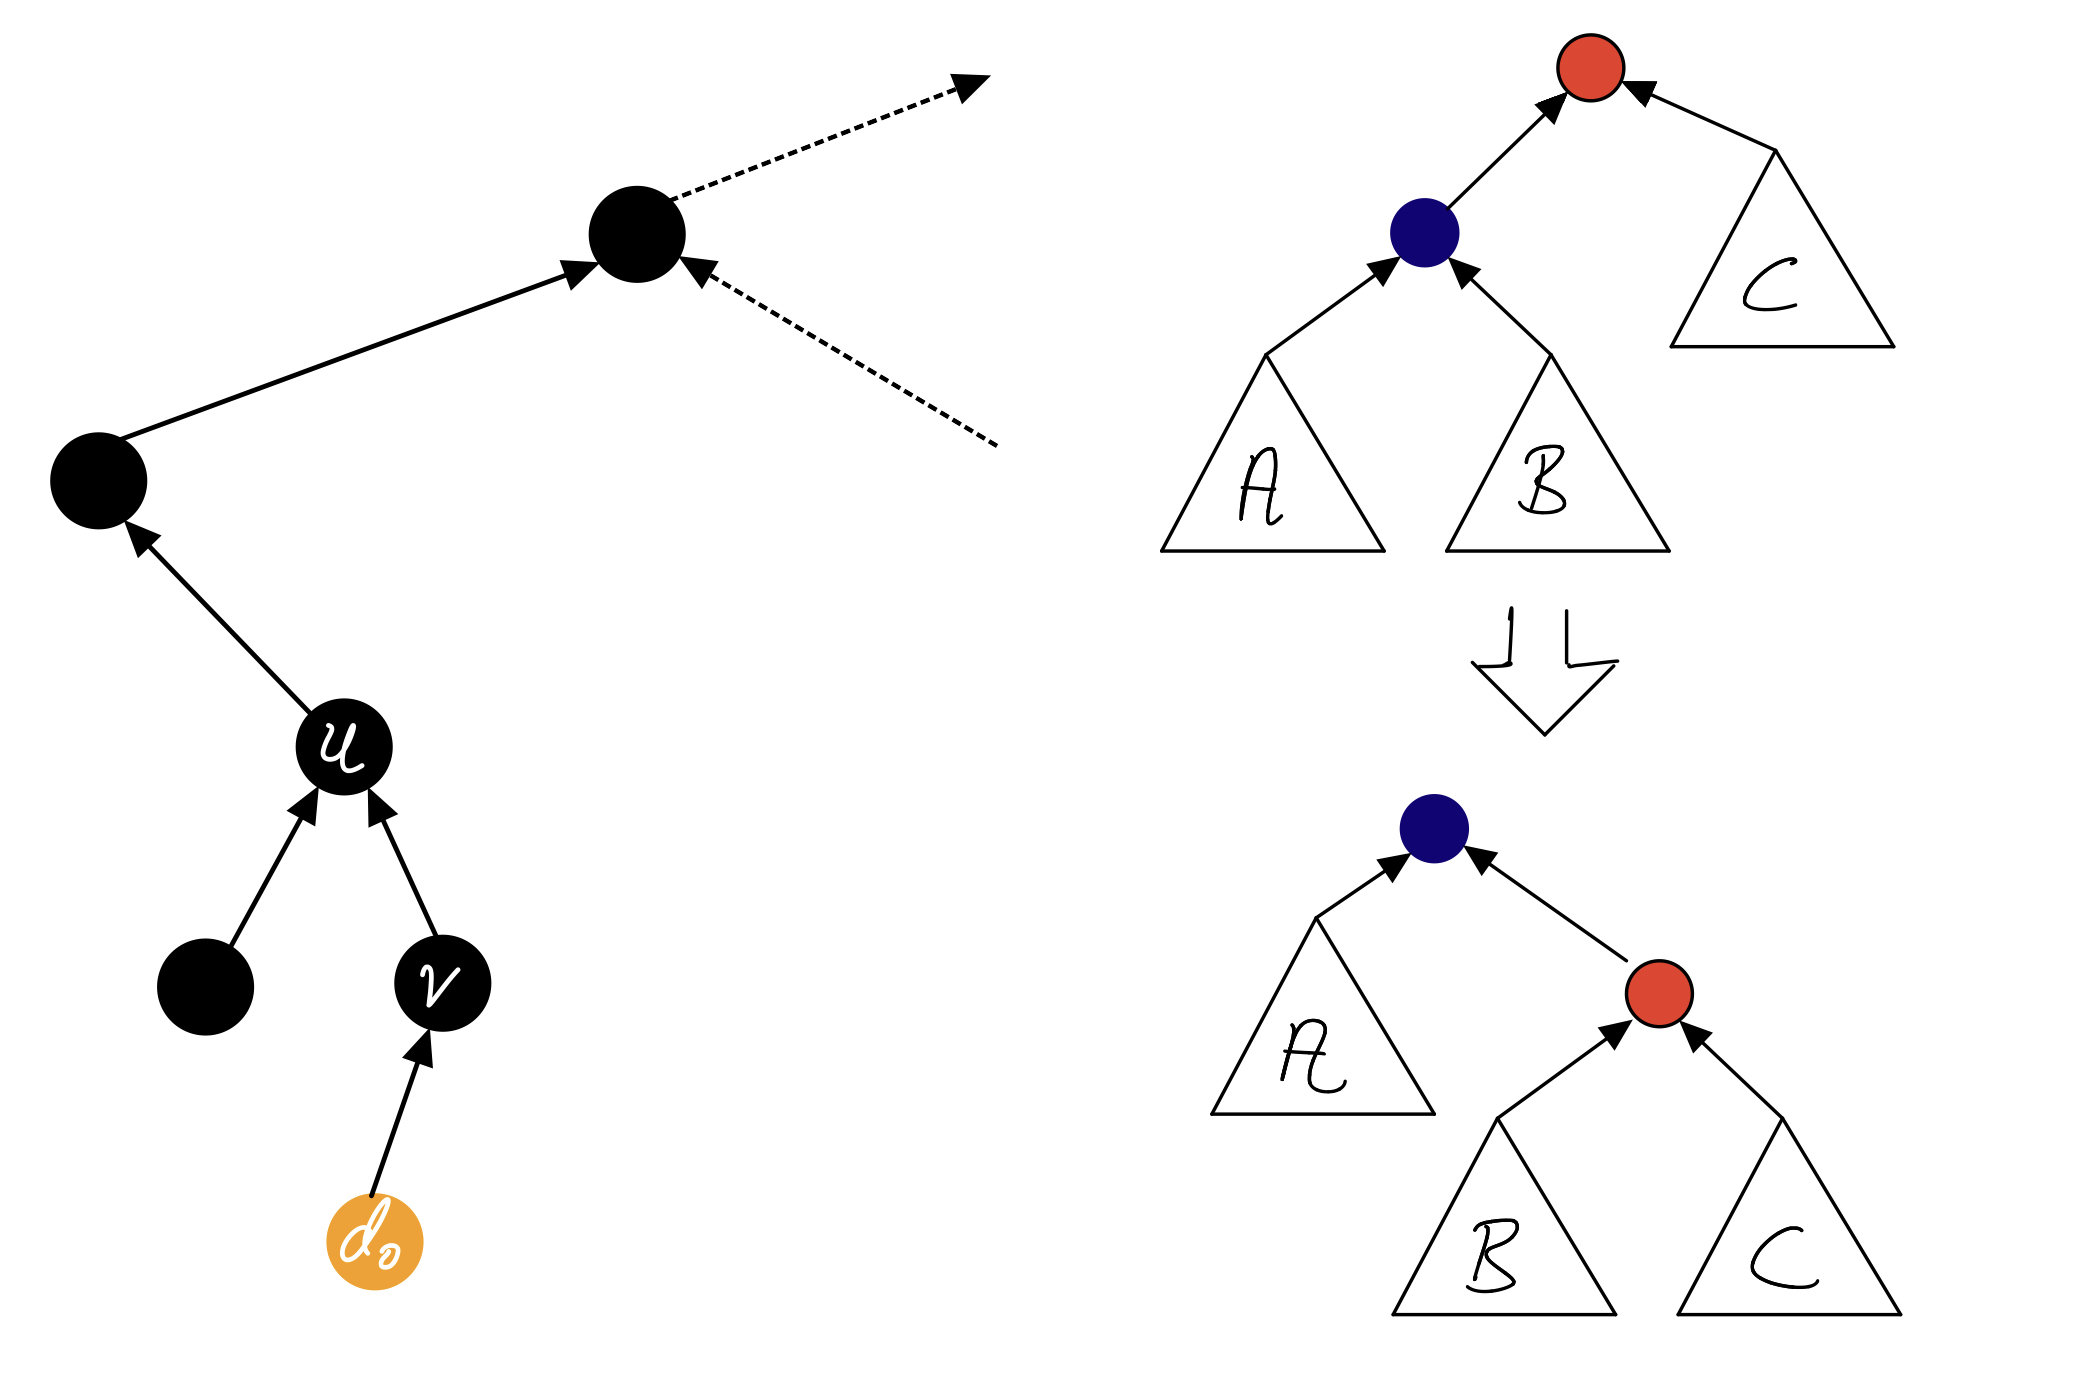
\includegraphics[scale=0.2]{./fig/PathCutOperation_lectureDynamicTree.jpeg}
    \caption{For $\textsc{Cut}(u,v)$, we insert a vertex $d_0$ as a leaf of either $u$ or $v$ to formally split $(u,v)$ into $(u,d_0)$ and $(d_0,v)$ (this is shown on the left). While this preserves that Search-Property, it will violate the Heap-Order. Thus, we need to use tree rotations (shown on the left) to push $d_0$ to the top of the tree $\mathcal{P}$ (the arrow between the tree rotations should point in both ways).}
    \label{fig:binaryTreeRotation}
\end{figure}

To ensure that the fields are correctly adjusted, we can make the $\Delta min(\cdot)$ values of the two vertices that are rotated equal to zero while ensuring that the tree is still \emph{field-preserving} by changing the $\Delta min(\cdot)$ fields of the (at most 3) roots of the subtrees to be rotated, and adapting the $\Delta cost(\cdot)$ fields of the two vertices to be rotated. Then, after the rotation, it is not hard to see that the tree is still \emph{field-preserving} and that the procedure applied in the second for-loop of the operation $\textsc{AddCost}(v, \Delta)$ can then just be applied to the two rotated vertices and the roots of their subtrees. This ensures that the fields are maintained correctly. All of these operations can be implemented in $O(1)$ time per tree rotation.

\paragraph{Implementing $\textsc{Link}(u,v)$.} Implementing $\textsc{Link}(u,v)$ could be done by reversing the process described above. We choose however a slightly different strategy: we insert a vertex $d_{\infty}$ with $ranNum(d_{\infty}) = n^{100}$ and make it a right child of $u$. We then find the root $r$ of the tree over the path containing $v$ (as a tail). Finally, we make $r$ a right child of $d_{\infty}$. It remains to use tree rotations to make $d_{\infty}$ a leaf in the tree.  Once this is accomplished, one can simply remove $d_{\infty}$ from the tree entirely (which can be seen as un-splitting two edges into $(u,v)$).  

\paragraph{Notes.} The operations $\textsc{Link}/ \textsc{Cut}$ can be implemented for almost all Balanced Binary Search Trees (especially the ones you have seen in your first courses on data structures). Thus, it is not hard to get a $O(\log n)$ worst-case time bound for all operations discussed above.

\section{Implementing Trees via Paths}

We now use the result from last section as a black box to obtain \Cref{thm:mainTheoremLinkCutTree}.

\paragraph{Path Decomposition.} For each rooted tree $T$, the idea is to decompose $T$ into paths. In particular, we decompose each $T$ into a collection of vertex-disjoint paths $P_1, P_2, \dots, P_k$ such that each internal vertex $v$ in $T$ has exactly one incoming edge in some $P_i$. We call the edges on some $P_i$  \emph{solid} edges and say that the other edges are \emph{dashed}. 

We maintain the paths $P_1, P_2, \dots, P_k$ using the data structure described in the last section. To avoid confusion, we use the prefix $P$ when we invoke operations of the path data structure, for example $\textsc{PFindRoot}(v)$ finds the root of $v$ in the path graph $P_i$ where $v \in P_i$.

\begin{figure}[!ht]
    \centering
    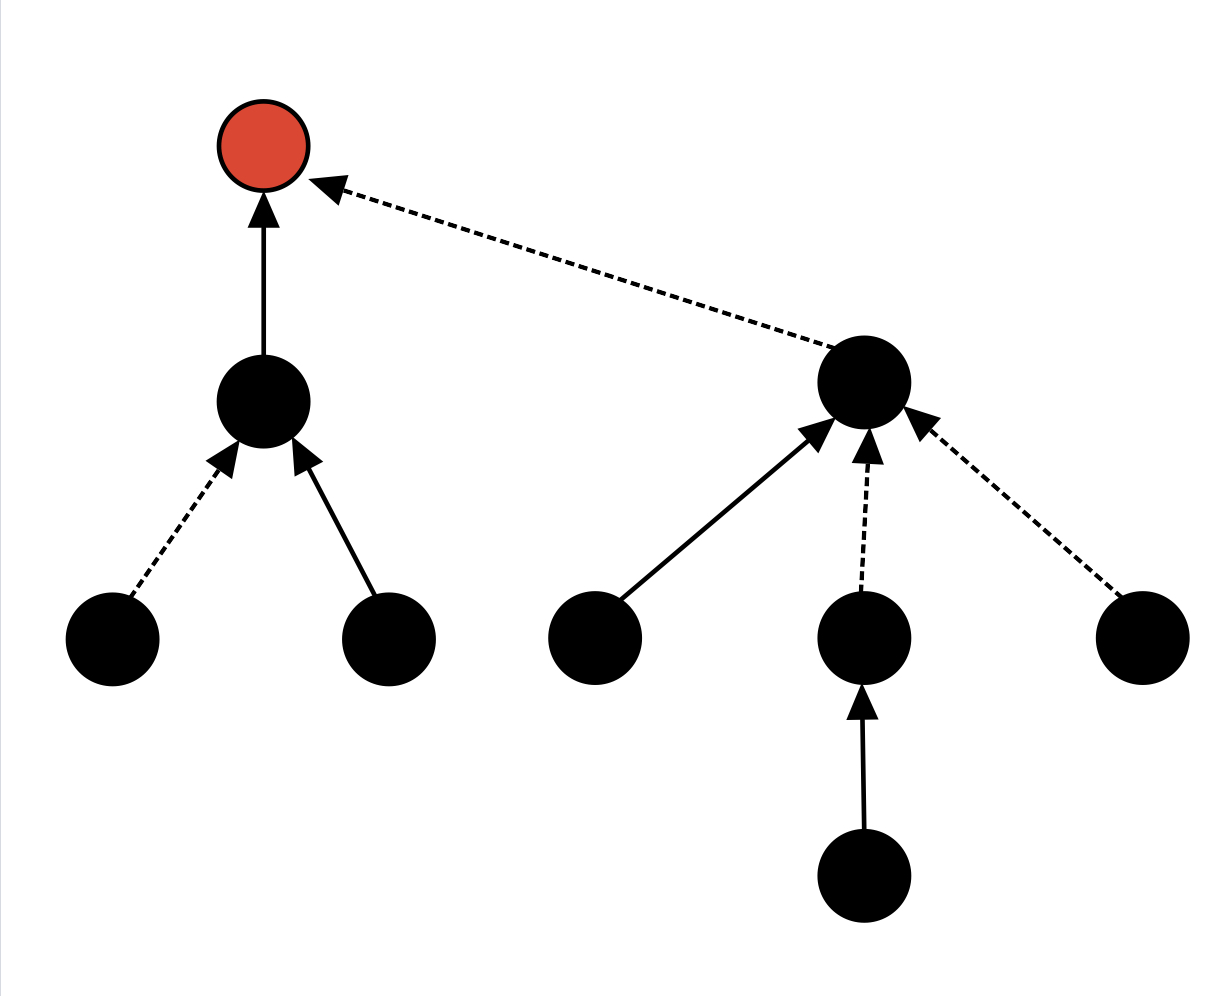
\includegraphics[scale=0.20]{./fig/HeavyLightDecomposition_lectureDynamicTree.jpeg}
    \caption{The dashed edges are the edges not on any path $P_i$. The collection of (non-empty) paths $P_1, P_2, \dots, P_k$ can be seen to be the maximal path segments of solid edges.}
\end{figure}

\paragraph{The $\textsc{Expose}(v)$ Operation.} We start by discussing the most important operation of the data structure that will be used by all other operations internally: the operation $\textsc{Expose}(v)$. This operation flips solid/dashed edges such that after the procedure the path from $v$ to its tree root in $G$ is solid (possibly as a subpath in the path collection). Below you can find an implementation of the procedure $\textsc{Expose}(v)$. 

\begin{algorithm}
  \SetAlgoLined
  $w \gets v$.\\
  \While{$(w' = parent_G(\textsc{PFindRoot}(w))) \neq NULL$}{
    Invoke $\textsc{PCut}(z,w')$ for the solid edge $(z,w')$ incoming to $w'$.\\
    $\textsc{PLink}(w,w')$.\\
    $w \gets w'$.\\
  }
  \caption{\textsc{Expose}(v)}
\end{algorithm}

\paragraph{Implementing Operations via $\textsc{Expose}(v)$.} We can now implement link-cut tree operations by invoking $\textsc{Expose}(v)$ and then forwarding the operation to the path data structure. 
\begin{algorithm}[H]
  \SetAlgoLined
  $\textsc{Expose}(v)$; $\textsc{PAddCost}(v, \Delta)$
  \caption{$\textsc{AddCost}(v, \Delta)$}
\end{algorithm}
\begin{algorithm}[H]
  \SetAlgoLined
  $\textsc{Expose}(v)$; \Return $\textsc{PFindMin}(v)$
  \caption{\textsc{FindMin}(v)}
\end{algorithm}
\begin{algorithm}[H]
  \SetAlgoLined
  $parent_G(u) \gets v$\;
  \lIf{$v$ has an incoming solid edge $(z,v)$}{
    $\textsc{PCut}(z,v)$
  }
  $\textsc{PLink}(u,v)$
  \caption{\textsc{Link}(u,v)}
\end{algorithm}
\begin{algorithm}[H]
  \SetAlgoLined
  $\textsc{Expose}(u)$; $parent_G(u) \gets NULL$; $\textsc{PCut}(u,v)$\;
   \lIf{$v$ has other incoming edge $(z,v)$}{$\textsc{PLink}(z,v)$}
  \caption{\textsc{Cut}(u,v)}
\end{algorithm}

\paragraph{Analysis.} All of the operations above can be implemented using a single $\textsc{Expose}(\cdot)$ operation plus $O(1)$ operations on paths. Since path operations can be executed efficiently, our main task is to bound the run-time of $\textsc{Expose}(\cdot)$. More precisely, since each iteration of $\textsc{Expose}(\cdot)$ also runs in time $O(\log n)$, the total number of while-loop iterations in $\textsc{Expose}(\cdot)$.

To this end, we introduce a dichotomy over the vertices in $G$. We let $parent_G(v)$ denote the unique parent of $v$ in $G$ and let $size_G(v)$ denote the number of vertices in the subtree rooted at $v$ (including $v$). 

\begin{definition}
Then, we say that an edge $(u,v)$ is \emph{heavy} if $size_G(u) > size_G(v)/2$. Otherwise, we say $(u,v)$ is \emph{light}. 
\end{definition}

It can now be seen that the number of \emph{light} edges on the $v$-to-root path for any $v$ is at most $\lg n$: every time we follow a light edge $(w,w')$, i.e. when $size_G(w') > 2 size_G(w)$, we double the size of the subtree so after taking more than $\lg n$ such edges, we have $> 2^{\lg n} = n$ vertices in the graph (which is a contradiction).

Thus, when $\textsc{Expose}(\cdot)$ runs for many iterations, it must turn many \emph{heavy} edges \emph{solid} (this is also since each vertex has at most one incoming heavy edge, so when we make a heavy edge solid, we also don't make any other heavy edge solid). 

\begin{claim}
Each update can only increase the number of dashed, heavy edges by $O(\log n)$. 
\end{claim}
\begin{proof}
First observe that every time $\textsc{Expose}(\cdot)$ is invoked, it turns at most $\lg n$ heavy edges from solid to dashed (since it has to visit a light edge to do so).

The only two operations that can cause additional dashed, heavy edges are $\textsc{Link}(u,v)$ and $\textsc{Cut}(u,v)$ by toggling heavy/light. For $\textsc{Link}(u,v)$, we observe that only the vertices on the $v$-to-root path increase their sizes. Since there are at most $\lg n$ light edges on this path that can turn heavy, this increases the number of dashed, heavy edges by at most $\lg n$. 

The case for $\textsc{Cut}(u,v)$ is almost analogous: only vertices on the $v$-to-root path decrease their sizes which can cause any heavy edge on such a path to become light, and instead for a sibling of such a vertex might becomes heavy. But there can be at most $\lg n$ such new heavy edges, otherwise the total size of the tree must exceed again $n$ which leads to a contradiction.
\end{proof}

Thus, after $m$ updates, we have created at most $O(m \log n)$ dashed heavy edges. The iterations of $\textsc{Expose}(\cdot)$ either visit a dashed light edge (at most $\ln n$ of them), or consumes a dashed heavy edge, i.e. turning them .
We conclude that after $m$ updates, the while-loop in $\textsc{Expose}(\cdot)$ runs for at most $O(m \log n)$ iterations, \emph{in total}, i.e. summed across the updates so far. Each iteration can be implemented in $O(\log n)$ expected time. This dominates the total running time and proves \Cref{thm:mainTheoremLinkCutTree}.

\section{Fast Blocking Flow via Dynamic Trees}

Recall from \Cref{sec:findBlockingFlows} that computing blocking flows in a level graph $L$ from a vertex $s$ to $t$ can be done by successively running $\textsc{DFS}(s)$ and routing flow along the $s$-$t$ path found if one such path exists and otherwise we know that we have found a blocking flow. 

We can now speed-up this procedure by storing the DFS-tree explicitly as a dynamic tree. To simplify exposition, we transform $L$ to obtain a graph $\textsc{Transform}(L)$ that has capacities on vertices instead of edges. To obtain $\textsc{Transform}(L)$, we simply split each edge in $L$ and assign the edge capacity to the mid-point vertex while assigning capacity $\infty$ to all vertices that were already in $L$. This creates an identical flow problem with at most $O(m)$ vertices and edges.

\begin{figure}[!ht]
    \centering
    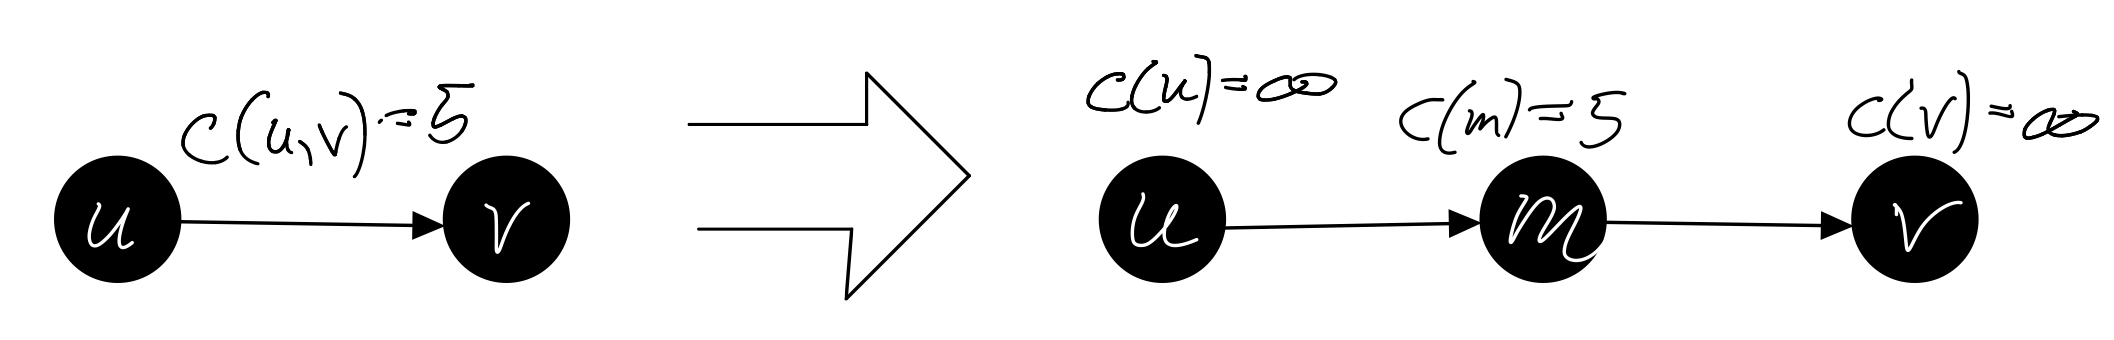
\includegraphics[scale=0.2]{./fig/TransformToVertCaps_lectureDynamicTree.jpeg}
    \caption{Each edge $(u,v)$ with capacity $c(u,v)$ is split into two edges $(u,m)$ and $(m,v)$. The capacity is then on the vertex $m$.}
    \label{fig:my_label}
\end{figure}

Finally, we give the new pseudo-code for the blocking flow procedure below.

\begin{algorithm}[H]
  \SetAlgoLined
  $H \leftarrow \textsc{Transform}(L)$\;
  $\textsc{LC-Tree} \gets \textsc{Initialize}(H)$\;
  
  \While{$s \in H$}{
    $u \gets \textsc{LC-Tree}.\textsc{FindRoot}(s)$\;
    \eIf{there is an edge $(u,v) \in H$}{
        $\textsc{LC-Tree}.\textsc{Link}(u,v)$\;
        \If{$v = t$}{
            $(w, c) \gets \textsc{LC-Tree}.\textsc{FindMin}(s)$\;
            $\textsc{LC-Tree}.\textsc{AddCost}(s, - c)$\;
            Remove $w$ and all its incident edges from $H$ and $\textsc{LC-Tree}$ (via $\textsc{Cut}(\cdot)$).
        }
    }{
        Remove $u$ and all its incident edges from $H$ and $\textsc{LC-Tree}$ (via $\textsc{Cut}(\cdot)$).
    }
  }
  Construct $\ff$ by setting for each edge $(u,v)$ of $L$, with mid-point $m$ in $\textsc{Transform}(L)$, the flow equal to $c(m)$ minus the cost on $m$ just before it was removed from $H$.
  \caption{\textsc{FindBlockingFlow}(s, t, L)}
\end{algorithm}

\begin{claim}
The running time of $\textsc{FindBlockingFlow}(s, t, L)$ is $O(m \log^2 n + |V|)$.
\end{claim}
\begin{proof}
Each edge $(u,v)$ in the graph $\textsc{Transform}(L)$ enters the link-cut tree at most once (we only invoke $\textsc{Cut}(u,v)$ when we delete $(u,v)$ from $H$). 

Next, observe that the first $if$-case requires $O(1 + \#edgesDeletedFromH)$ many tree operations. The $else$-case requires $O(\#edgesDeletedFromH)$ many tree operations. 

But each edge is only deleted once from $H$, thus we have a total of $O(m)$ tree operations over all iterations. Since each link-cut tree operation takes amortized expected time $O(\log^2 n)$, we obtain the bound on the total running time. 
\end{proof}

The correctness of this algorithm follows almost immediately using that the level graph $L$ (and therefore $\textsc{Transform}(L)$) is an ayclic graph.

%%% Local Variables:
%%% mode: latex
%%% TeX-master: "main"
%%% End: